\documentclass[]{article}
\usepackage[a4paper, total={7in, 9in}]{geometry}

%opening
\title{pRF simulation with Compressive Spatial Summation model}
\author{Arash Ashrafnejad}

\usepackage{graphicx}
\usepackage{float}

\begin{document}

\maketitle
\newpage


\section{Introduction}
This is the introduction \footnote{footnotes working fine}. Refer $\int_{0}^{1} f(x) dx$ to Figure \cite{Kay2013}

\begin{equation}
	\int_{0}^{1} f(x) dx
\end{equation}
\begin{equation}
\int_{0}^{1} f(x) dx
\end{equation}


\begin{figure}[htp]
	\centering
	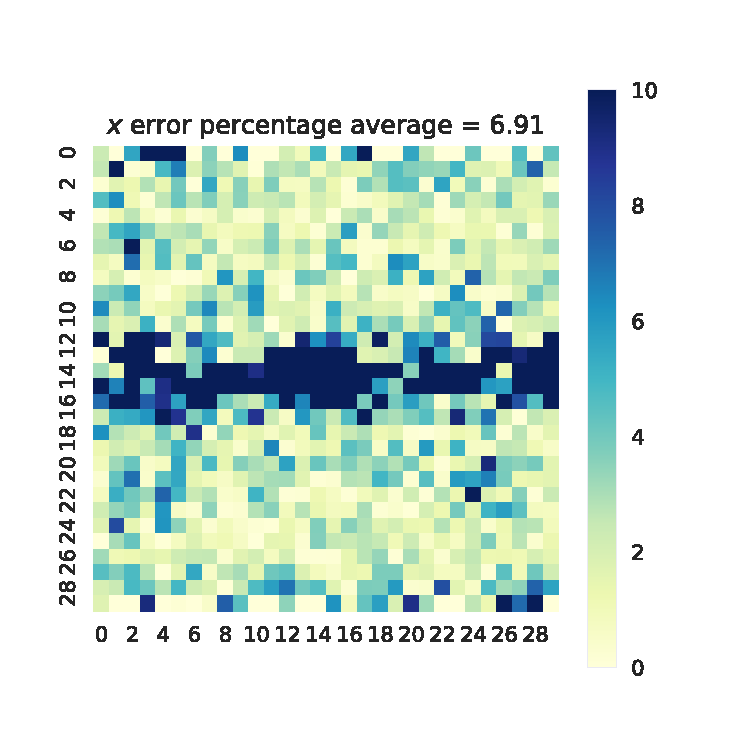
\includegraphics[width=.32\textwidth]{x_5}
	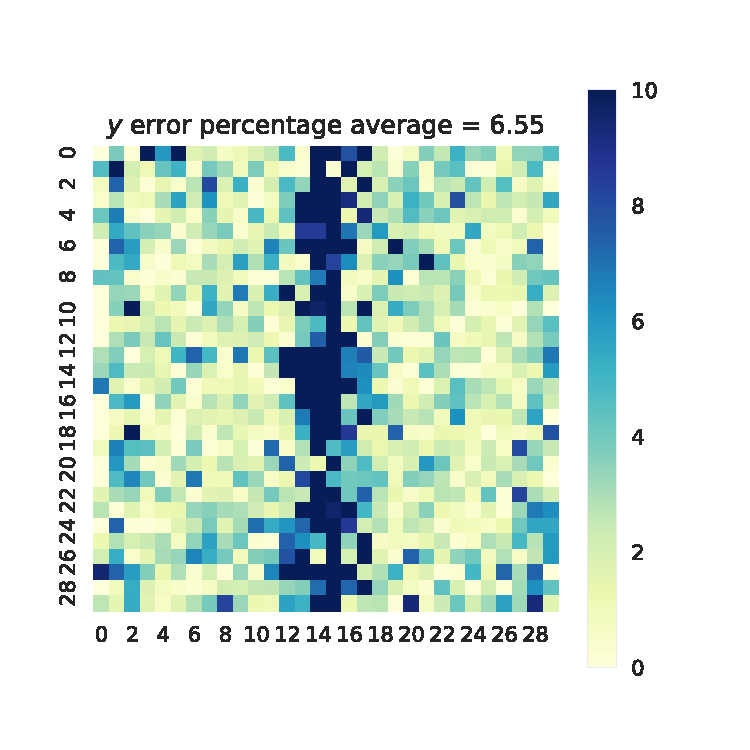
\includegraphics[width=.32\textwidth]{y_5}
	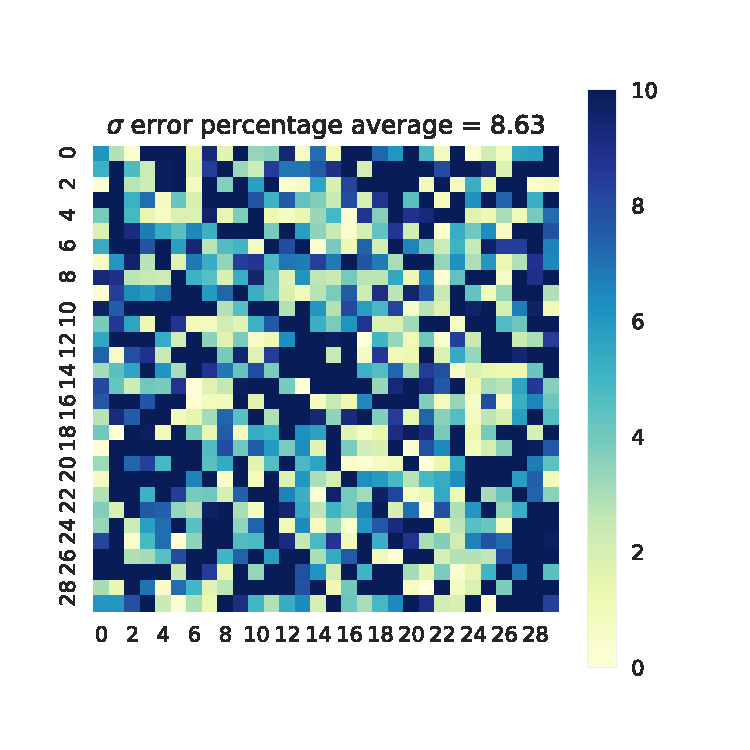
\includegraphics[width=.32\textwidth]{sigma_5}
	\vspace{-0.5cm}
	\caption{CSS model with exponent $n=0.5$}
\end{figure}
\begin{figure}[htp]
	\centering
	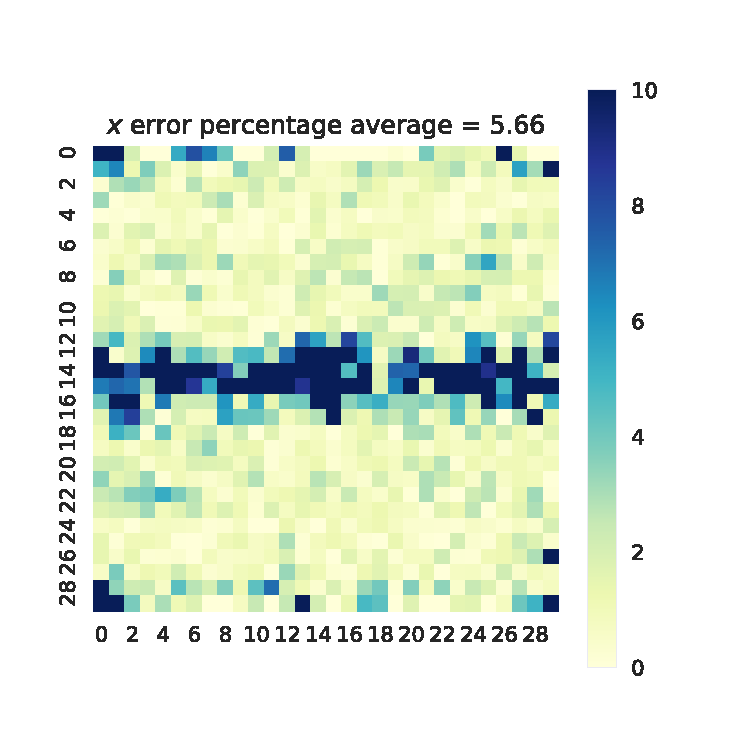
\includegraphics[width=.32\textwidth]{x_6}
	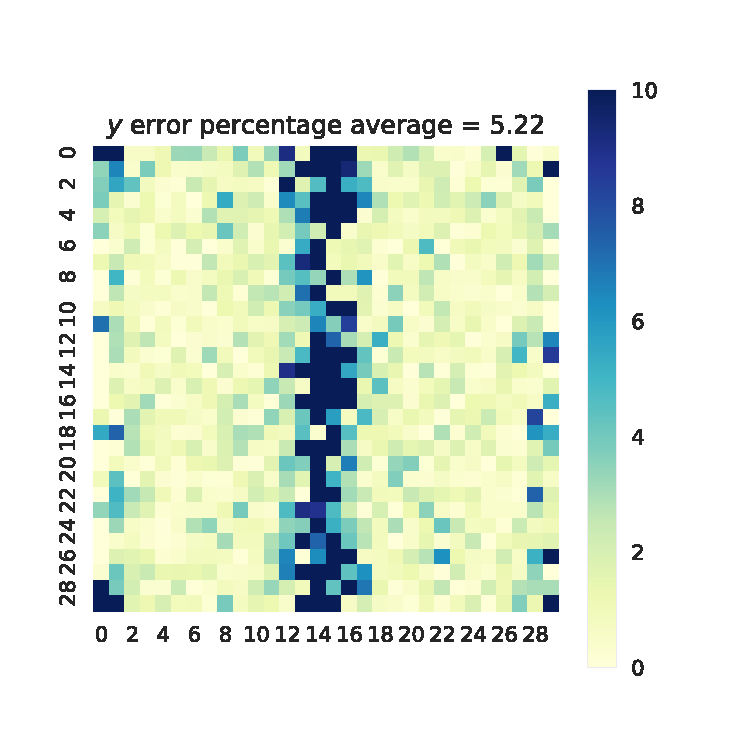
\includegraphics[width=.32\textwidth]{y_6}
	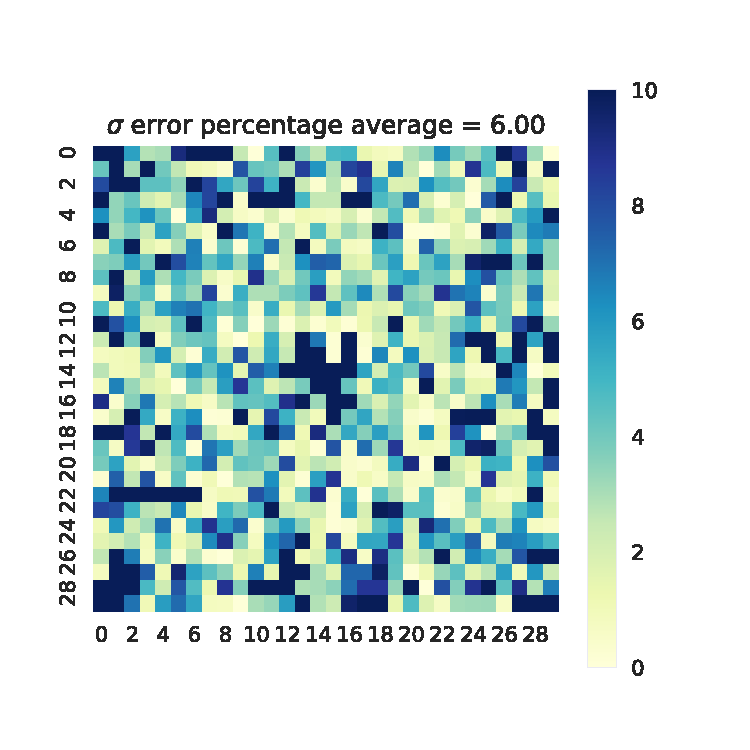
\includegraphics[width=.32\textwidth]{sigma_6}
	\vspace{-0.5cm}
	\caption{CSS model with exponent $n=0.6$}
\end{figure}
\begin{figure}[htp]
	\centering
	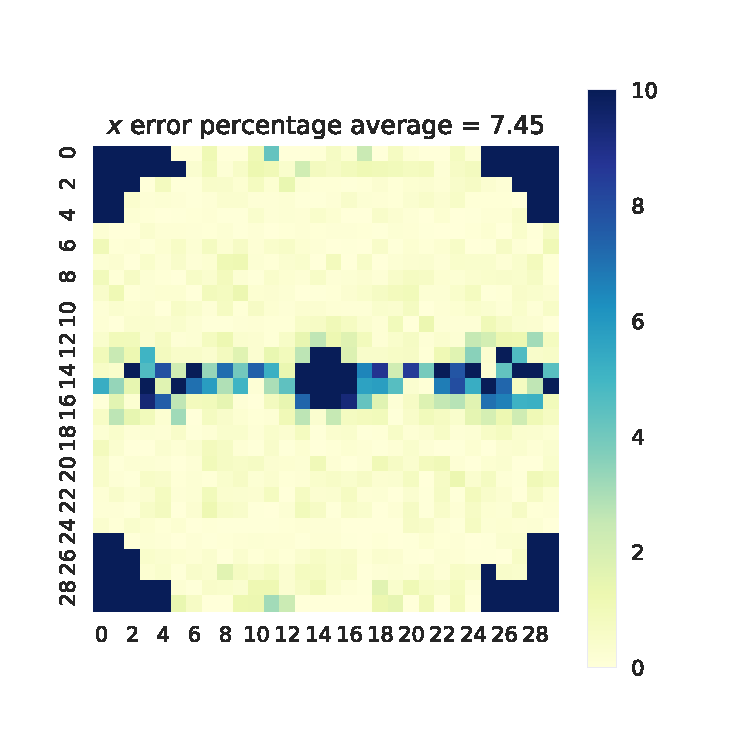
\includegraphics[width=.32\textwidth]{x_7}
	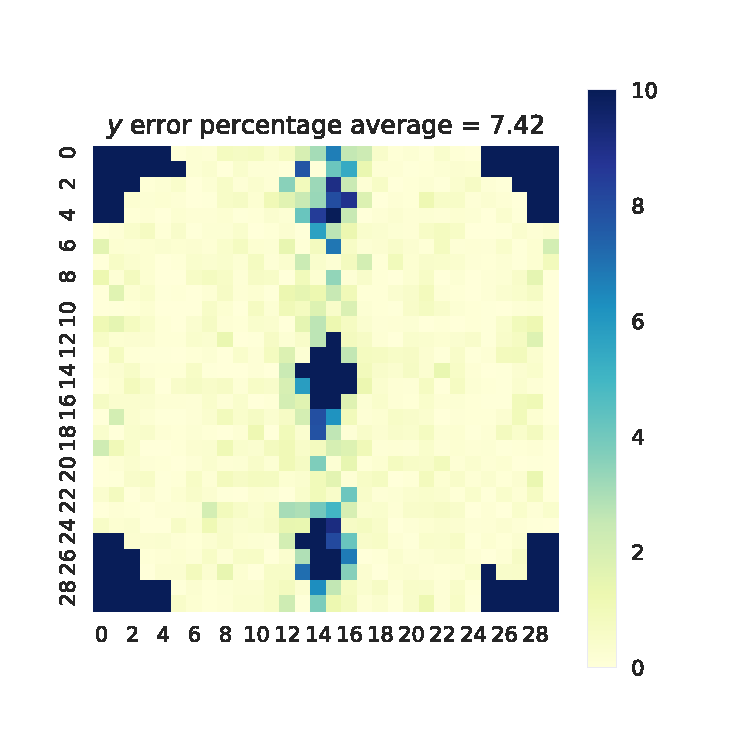
\includegraphics[width=.32\textwidth]{y_7}
	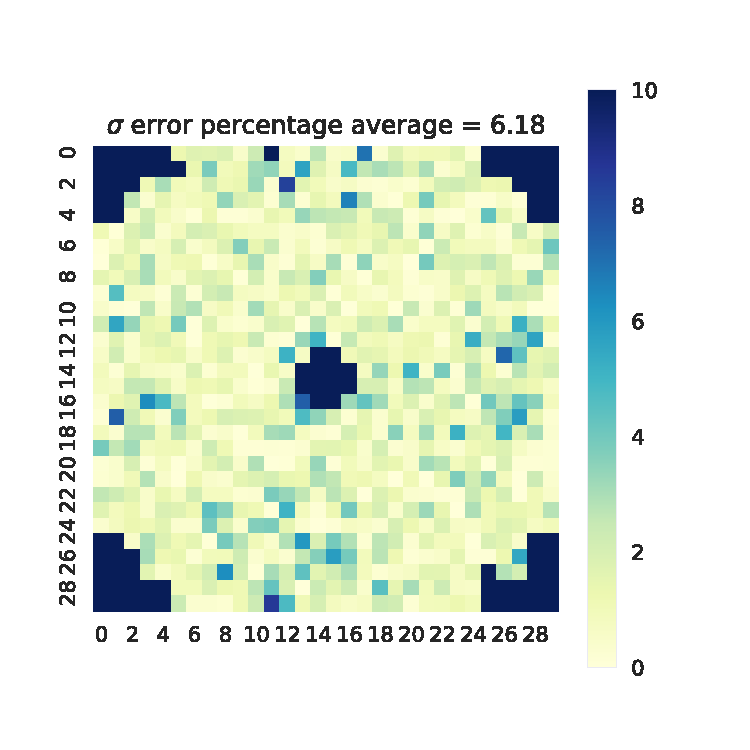
\includegraphics[width=.32\textwidth]{sigma_7}
	\vspace{-0.5cm}
	\caption{CSS model with exponent $n=0.7$}
\end{figure}
\begin{figure}[htp]
	\centering
	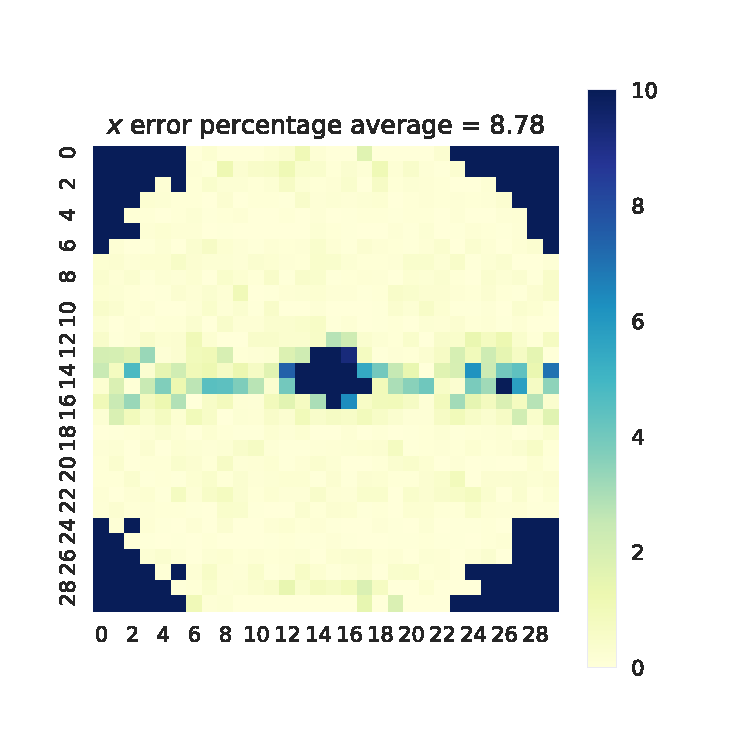
\includegraphics[width=.32\textwidth]{x_9}
	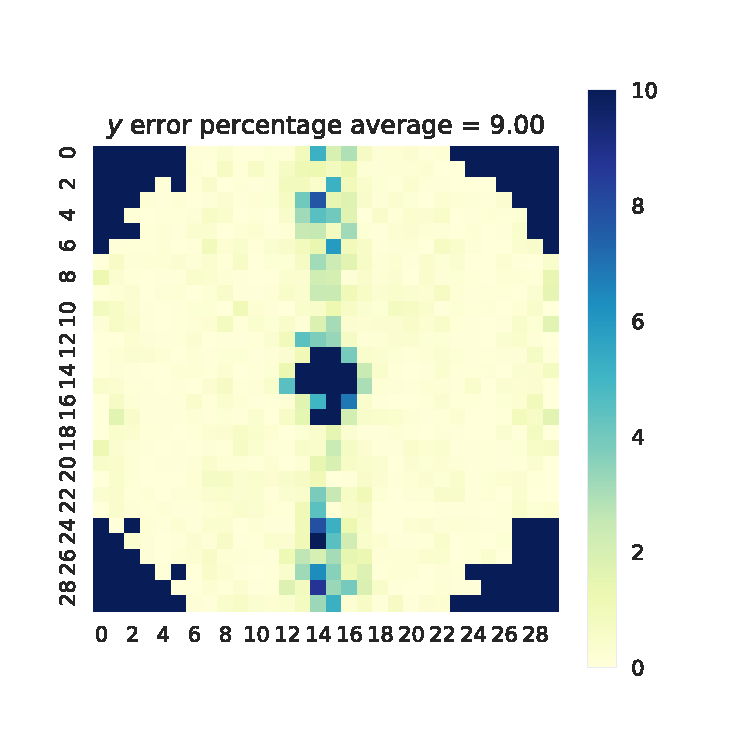
\includegraphics[width=.32\textwidth]{y_9}
	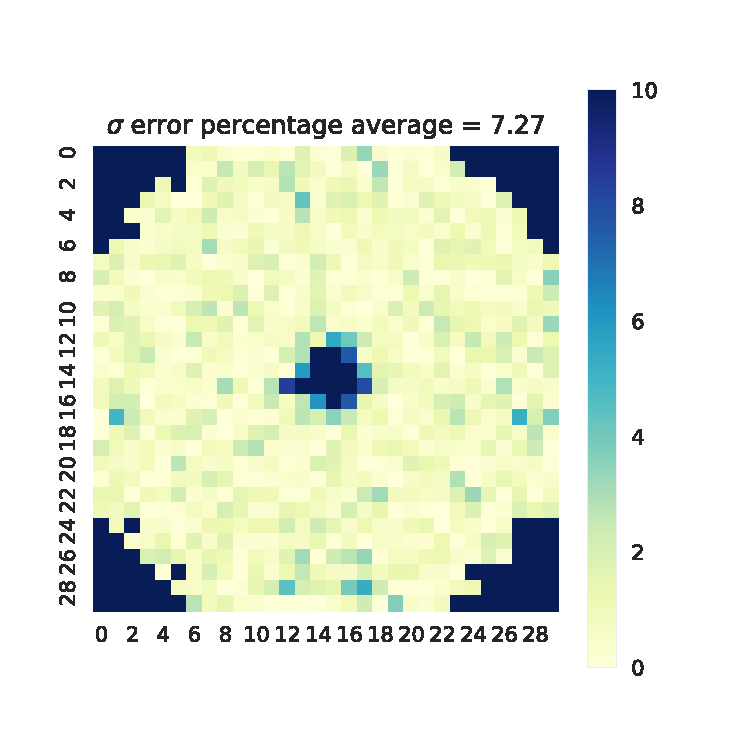
\includegraphics[width=.32\textwidth]{sigma_9}
	\vspace{-0.5cm}
	\caption{CSS model with exponent $n=0.9$}
\end{figure}
\begin{figure}[htp]
	\centering
	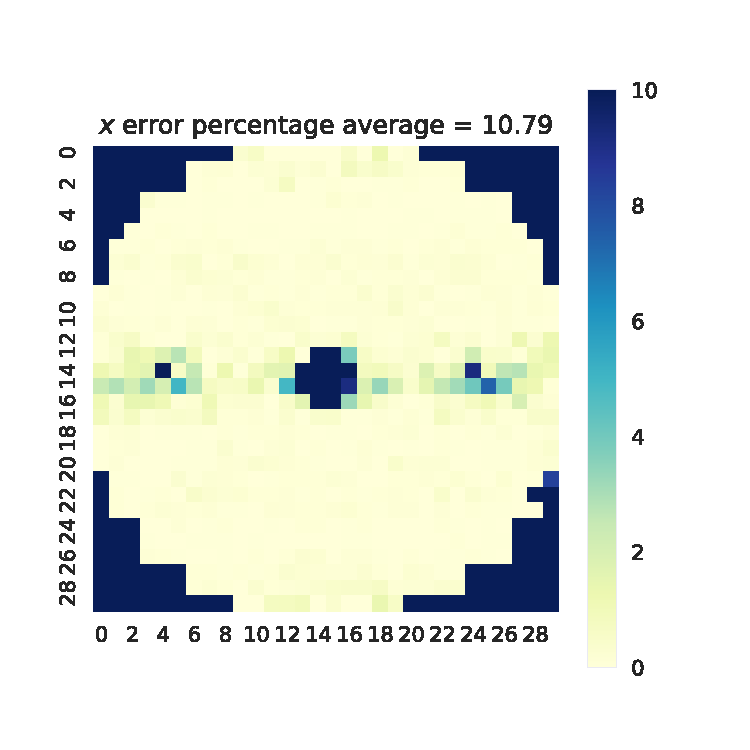
\includegraphics[width=.32\textwidth]{x_10}
	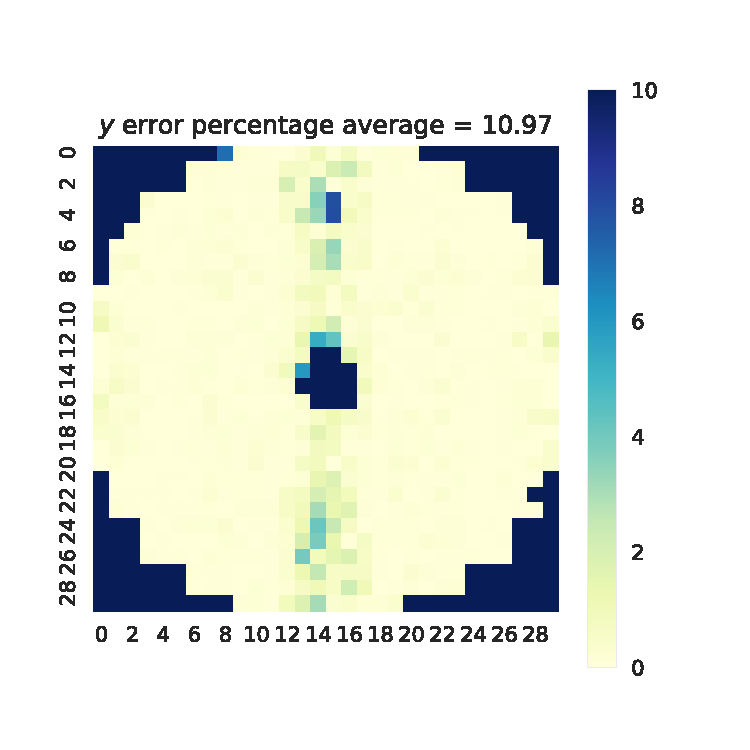
\includegraphics[width=.32\textwidth]{y_10}
	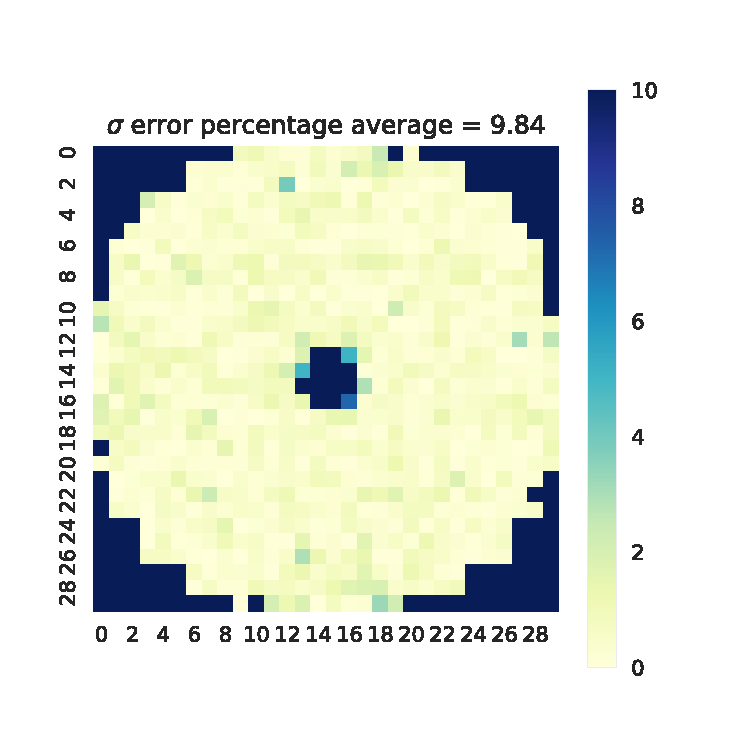
\includegraphics[width=.32\textwidth]{sigma_10}
	\vspace{-0.5cm}
	\caption{Linear model $n=1.0$}
\end{figure}









\bibliographystyle{unsrt}
\bibliography{refs}
\end{document}
